\chapter{Resultados}
\label{cap:result}
Para sabermos se o protótipo atingiu nossos objetivos é preciso analisar quatro pontos importantes: sua capacidade de transmissão em longo alcance, sua capacidade de lidar com altas interferências ao longo do trajeto, seu consumo energético e seu custo de produção.

% ---
\section{Análise de Transmissão dos Pacotes}
\label{result:transmissao}
Foi executado um teste de transmissão de pacotes com o objetivo de verificar a capacidade de transmissão em um longo alcance em um ambiente com altas interferências. O experimento foi realizado no bloco dos professores do IFPB - Campus Campina Grande, onde o \textit{end node} ficou posicionado no laboratório GComPi, localizado no subsolo, enquanto o \textit{gateway} ficou em um espaço diferente, no Laboratório Assert, no térreo do prédio, com cerca de sessenta metros de distância entre os dispositivos, e contanto com obstáculos variados à comunicação, como paredes densas, laje, objetos metálicos e equipamentos eletrônicos. Na figura \ref{fig:experiment-01} podemos ver a distância entre o gateway e o end node, respectivamente, A e B.

\begin{figure}[H]
  \centering
  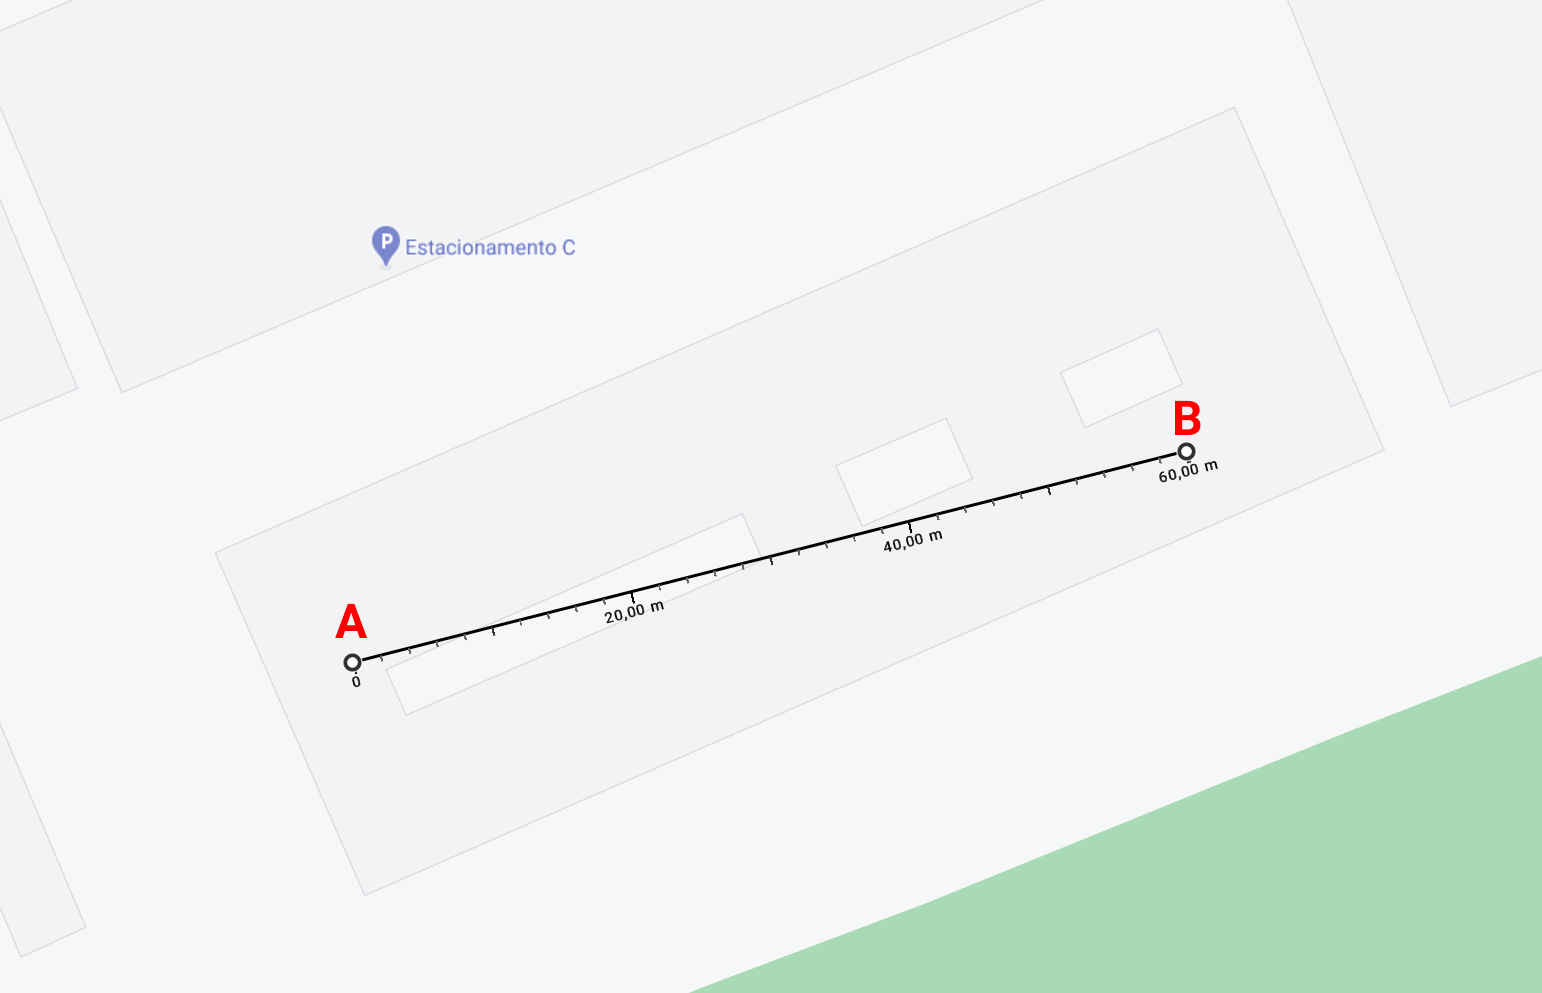
\includegraphics[width=.80\textwidth]{assets/experiment-01.png} 
  \caption{Distância aproximadas entre os dispositivos (Adaptada do Google Maps).}
  \label{fig:experiment-01} 
\end{figure}

Os dispositivos ficaram funcionando por alguns dias, 24 horas por dias, realizando envios contínuos de pacotes em intervalos de cinco minutos. O gráfico na figura \ref{fig:21-04-2020-pdr-rssi} apresenta a taxa de entrega de pacote, PDR, por horas, das coletas realizadas no dia 21 de abril de 2020. A média geral da PDR foi de 78.82\%, um valor agradável, no entanto, em alguns momentos a PDR ficou em torno de 20\%, o que pode ter sido ocasionado por modificações no perfil de multi-percurso do ambiente, obstáculos temporários ou presença de fontes de interferência. Considerando a taxa de transmissão de pacote utilizada, com PDR de 20\% ainda é possível obter uma nova informação a cada 25 minutos, em média, o que é suficiente para a realização do monitoramento de temperatura e umidade, que são grandezas que variam lentamente.

\begin{figure}[H]
  \centering
  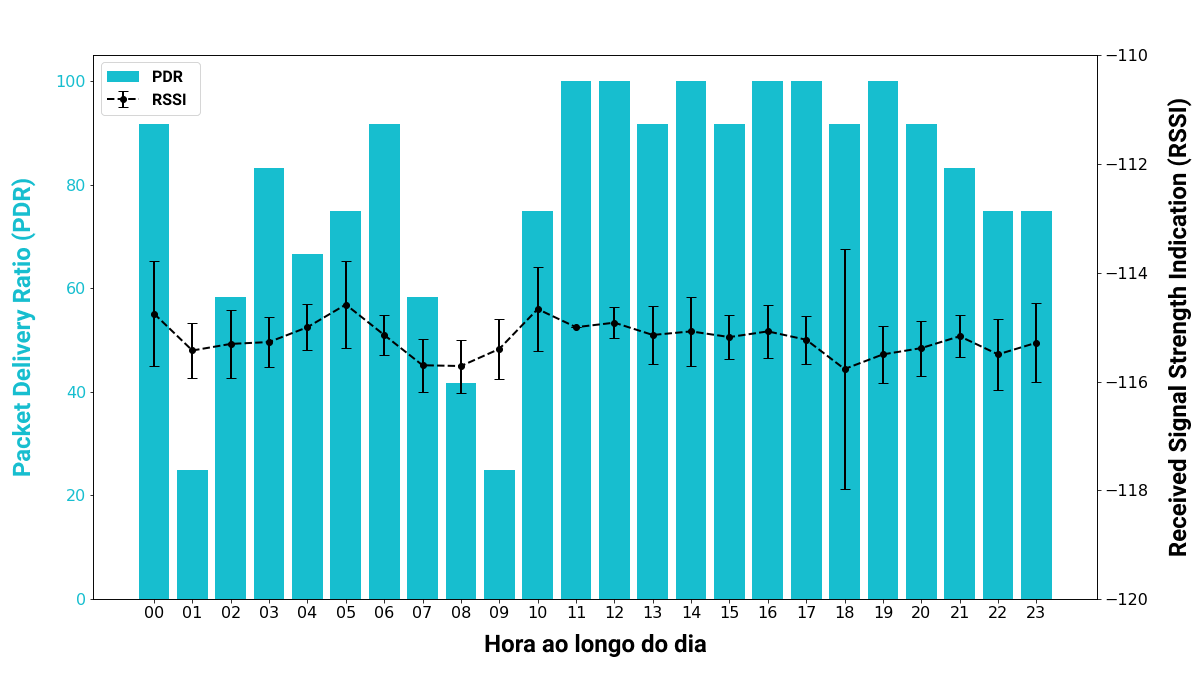
\includegraphics[width=.80\textwidth]{assets/21-04-2020-pdr-rssi.png} 
  \caption{Percentual de entrega dos pacotes em barras e indicador de intensidade do sinal recebido em linha. (Autoral).}
  \label{fig:21-04-2020-pdr-rssi} 
\end{figure}

% ---
\section{Análise do Consumo Energético}
\label{result:consumo}

% ---
\section{Análise do Custo}
\label{result:custo}
Todas as compras dos equipamentos foram realizadas no Brasil e em baixa quantidade, o que acaba deixando o protótipo mais caro do que em comparação a um produto produzido em massa, que acaba tendo uma redução considerável do seu custo. Tendo isto em mente, podemos analisar a tabela \ref{tab:costs-2-proto}, representando o custo da cada peça encontrada no Brasil e na China para montar uma unidade do segundo protótipo apresentado na sessão \ref{metod:end-node:2-proto}.

\begin{table}[H]
  \centering 
  \scalebox{1} {
    \begin{tabular}{l | l | l}
    \textbf{Componente}&\textbf{Preço no Brasil}&\textbf{Preço na China}\\[5pt] \hline
    &&\\
    Um ATmega328&R\$ 19,90&R\$ 9,12 \\[5pt]
    Um LoRa RFM95W 915Mhz&R\$ 56,00&R\$ 20,99 \\[5pt]
    Um Bateria 18650 3000mAh&R\$ 19,90 &R\$ 17,65 \\[5pt]
    Um Cristal Oscilador 16mhz&R\$ 01,47&R\$ 00,46 \\[5pt]
    Um Capacitor de cerâmica 100pF&R\$ 00,05&R\$ 00,04 \\[5pt]
    Dois Capacitor de cerâmica 22pF&R\$ 00,22&R\$ 00,08 \\[5pt]
    Dois Resistores de 10k Ohms&R\$ 00,12&R\$ 00,06 \\
    &&\\ \hline
    &&\\
    \textbf{Total}&R\$ 97,66&R\$ 48,40 \\[5pt]
    \end{tabular}
  }
  \caption{Custos referente as peças do segundo protótipo do \textit{end node} (autoral).}
  \label{tab:costs-2-proto}
\end{table}
  